\documentclass[11pt,a4paper]{article}

\usepackage[T1]{fontenc}
\usepackage[utf8]{inputenc}
\usepackage{lmodern}
\usepackage[margin=2.3cm]{geometry}
\usepackage{amsmath,amssymb,booktabs,enumitem,microtype}
\usepackage{tikz}
\usetikzlibrary{arrows.meta}
\usepackage[hidelinks]{hyperref}

\setlength{\parindent}{0pt}
\setlength{\parskip}{0.5em}
\setlist{itemsep=2pt,topsep=4pt}

\newcommand{\dd}{\mathrm{d}}
\newcommand{\A}{\mathcal{A}}
\newcommand{\vr}{\mathbf{r}}
\newcommand{\vp}{\mathbf{p}}
\newcommand{\vv}{\mathbf{v}}
\newcommand{\vT}{\mathbf{T}}

\title{Hamilton's Principle:\\
From Stationary Action to Wavefronts and Rays}
\author{A second lecture on variational mechanics}
\date{}

\begin{document}

\maketitle

\textbf{Duration:}
45 minutes, with optional instructor calculations afterward.

\textbf{Background:}
The preceding lecture on first variations and the Euler--Lagrange
equation. Introduce gradients as normals to level sets if needed.

\textbf{Scope:}
One particle with constant mass in Cartesian coordinates.
Two spatial dimensions make the geometry visible; the formulas
also work in one or three dimensions.

\textbf{Central question:}
Can we describe a family of particle trajectories using a field
of surfaces, much as we describe light using wavefronts?

\begin{center}
\begin{tabular}{@{}ll@{}}
\toprule
Time & Topic \\
\midrule
0--5 min   & Stationary action and the wavefront picture \\
5--13 min  & The principal function and endpoint variations \\
13--19 min & Derive the Hamilton--Jacobi equation \\
19--29 min & Constant-action surfaces and free-particle rays \\
29--39 min & The optical--mechanical analogy \\
39--43 min & A glimpse of waves and quantum mechanics \\
43--45 min & Questions and the main chain of ideas \\
\bottomrule
\end{tabular}
\end{center}

\section*{0--5 minutes: From paths to wavefronts}

Draw circular ripples and radial lines on the board.

\begin{quote}
In optics we can describe the same propagation using wavefronts
or rays. Could mechanics have a similar description?
\end{quote}

Recall the action functional:
\[
\A[\vr]
=
\int_{t_0}^{t_1}
L(\vr,\dot\vr,t)\,\dd t.
\]

Hamilton's principle states that a physical trajectory is
stationary under admissible variations with fixed endpoint
positions and times:
\[
\boxed{\delta\A=0.}
\]

The historical name is the principle of least action.
The general statement is stationarity; a physical path need not
give a minimum.

For the standard Lagrangian
\[
L=\frac12m|\dot\vr|^2-V(\vr,t),
\]
Euler--Lagrange gives, component by component,
\[
\frac{\dd}{\dd t}
\frac{\partial L}{\partial\dot r_i}
-
\frac{\partial L}{\partial r_i}
=0
\quad\Longrightarrow\quad
m\ddot\vr=-\nabla V.
\]

Today change the question:

\begin{quote}
Instead of varying paths between fixed endpoints, let the
endpoint move. What does the action of the classical path
tell us about that endpoint?
\end{quote}

\section*{5--13 minutes: Hamilton's principal function}

Fix an initial event \((\vr_0,t_0)\).
For each nearby final event \((\vr,t)\), consider a classical
trajectory joining them.

On a chosen smooth branch, define
\[
\boxed{
S(\vr,t;\vr_0,t_0)
=
\int_{t_0}^{t}
L(\vr_{\mathrm{cl}},
  \dot\vr_{\mathrm{cl}},\tau)\,\dd\tau.
}
\]

This is Hamilton's \textbf{principal function}.

The action \(\A[\vr]\) is a functional of arbitrary paths.
The principal function \(S\) is an ordinary function of the
endpoints, obtained by evaluating that functional on a
classical path.

If several classical trajectories reach the same final event,
there may be several branches of \(S\).
For now work where one branch is smooth.

Suppress the fixed initial event in the notation and write
\(S(\vr,t)\).

\subsection*{Moving the final position at fixed time}

Let \(\boldsymbol\eta(\tau)\) be the variation of the path at
fixed time.

The first-variation calculation from the previous lecture gives
\begin{align*}
\delta\A
&=
\int_{t_0}^{t}
\left(
L_{\vr}\cdot\boldsymbol\eta
+
L_{\dot\vr}\cdot\dot{\boldsymbol\eta}
\right)\dd\tau\\
&=
\left[\vp\cdot\boldsymbol\eta\right]_{t_0}^{t}
+
\int_{t_0}^{t}
\left(
L_{\vr}
-
\frac{\dd\vp}{\dd\tau}
\right)
\cdot\boldsymbol\eta\,\dd\tau,
\end{align*}
where
\[
\vp
:=
\frac{\partial L}{\partial\dot\vr}.
\]

On a classical path the integral vanishes.

The initial position is fixed, so
\[
\boldsymbol\eta(t_0)=0.
\]

At fixed final time,
\[
\boldsymbol\eta(t)=\delta\vr.
\]

Therefore,
\[
\delta S=\vp\cdot\delta\vr.
\]

Since the endpoint displacement is arbitrary,
\[
\boxed{\nabla S=\vp.}
\]

\begin{quote}
The spatial gradient of the accumulated classical action
is the momentum at arrival.
\end{quote}

\subsection*{Moving the final time too}

Now displace the final event by
\[
(\delta\vr,\delta t).
\]

The total endpoint displacement includes the extra time
along the path:
\[
\delta\vr
=
\boldsymbol\eta(t)
+
\dot\vr(t)\,\delta t.
\]

Hence
\[
\boldsymbol\eta(t)
=
\delta\vr-\dot\vr\,\delta t.
\]

The change of integration limit contributes \(L\,\delta t\).
Consequently,
\begin{align*}
\delta S
&=
\vp\cdot\boldsymbol\eta(t)+L\,\delta t\\
&=
\vp\cdot\delta\vr
+
\left(L-\vp\cdot\dot\vr\right)\delta t.
\end{align*}

Define the Hamiltonian by
\[
H:=\vp\cdot\dot\vr-L,
\]
with velocity expressed in terms of momentum when the
Legendre transform is invertible.

Thus,
\[
\boxed{
\dd S=\vp\cdot\dd\vr-H\,\dd t.
}
\]

Comparing this with the differential of an ordinary function,
\[
\dd S
=
\nabla S\cdot\dd\vr
+
\frac{\partial S}{\partial t}\dd t,
\]
we obtain
\[
\boxed{
\nabla S=\vp,
\qquad
S_t=-H.
}
\]

\section*{13--19 minutes: The Hamilton--Jacobi equation}

For our standard Lagrangian,
\[
\vp=m\dot\vr,
\qquad
\dot\vr=\frac{\vp}{m}.
\]

The Hamiltonian is
\begin{align*}
H
&=
\vp\cdot\dot\vr
-
\left(
\frac12m|\dot\vr|^2-V
\right)\\
&=
\frac{|\vp|^2}{m}
-
\frac{|\vp|^2}{2m}
+
V\\
&=
\frac{|\vp|^2}{2m}+V.
\end{align*}

Substitute \(\vp=\nabla S\) into \(S_t=-H\):
\[
\boxed{
\frac{\partial S}{\partial t}
+
\frac{|\nabla S|^2}{2m}
+
V(\vr,t)
=0.
}
\]

More generally,
\[
\boxed{
S_t+H(\vr,\nabla S,t)=0.
}
\]

This is the \textbf{Hamilton--Jacobi equation}.

\begin{quote}
A family of trajectories can be encoded in one scalar action
field. Its spatial derivatives give momenta; its time
derivative gives minus the Hamiltonian.
\end{quote}

One particular solution selects one family of trajectories.
Different initial data, or different branches, can describe
other families.

\section*{19--29 minutes: Action surfaces and rays}

\subsection*{Why the trajectories are normal to the surfaces}

At a \textbf{fixed time}, consider a regular level surface
\[
S(\vr,t)=\sigma.
\]

Let \(\vr(\lambda)\) be a curve lying inside that surface.

Differentiating its defining equation gives
\[
0
=
\frac{\dd}{\dd\lambda}S(\vr(\lambda),t)
=
\nabla S\cdot
\frac{\dd\vr}{\dd\lambda}.
\]

Thus \(\nabla S\) is perpendicular to every tangent of the
level surface.

For the standard kinetic energy,
\[
\boxed{
\dot\vr=\frac{\nabla S}{m}.
}
\]

Therefore trajectories cross the instantaneous constant-action
surfaces at right angles.

\textit{Condition for this statement.}
We use Cartesian coordinates and
\[
L=\frac12m|\dot\vr|^2-V,
\]
so momentum is parallel to velocity.

For a more general kinetic energy or a magnetic vector
potential, Euclidean orthogonality of velocity to these
surfaces does not automatically follow.

At points where \(\nabla S=0\), a regular normal direction
is not defined.

\begin{center}
\begin{minipage}{0.47\textwidth}
\centering
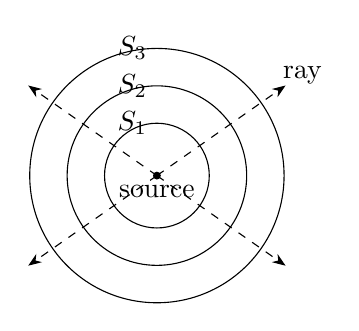
\begin{tikzpicture}[scale=0.95,>=Stealth]
  \foreach \radius in {0.7,1.2,1.7}{
    \draw (0,0) circle (\radius);
  }
  \foreach \angle in {35,145,215,325}{
    \draw[->,dashed] (0,0)--(\angle:2.1);
  }
  \fill (0,0) circle (1.5pt);
  \node[below] at (0,0) {source};
  \node[left] at (90:0.7) {$S_1$};
  \node[left] at (90:1.2) {$S_2$};
  \node[left] at (90:1.7) {$S_3$};
  \node[above right] at (35:1.9) {ray};
\end{tikzpicture}

\small
Point-source action surfaces at fixed time.
\end{minipage}
\hfill
\begin{minipage}{0.47\textwidth}
\centering
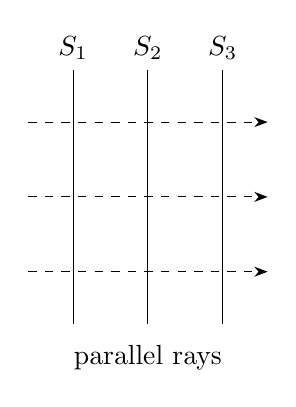
\begin{tikzpicture}[scale=0.95,>=Stealth]
  \foreach \x in {-1,0,1}{
    \draw (\x,-1.7)--(\x,1.7);
  }
  \foreach \y in {-1,0,1}{
    \draw[->,dashed] (-1.6,\y)--(1.6,\y);
  }
  \node[above] at (-1,1.7) {$S_1$};
  \node[above] at (0,1.7) {$S_2$};
  \node[above] at (1,1.7) {$S_3$};
  \node[below] at (0,-1.85) {parallel rays};
\end{tikzpicture}

\small
A plane-front family.
\end{minipage}
\end{center}

\subsection*{Worked example: A free particle from one point}

Set \(V=0\), fix \((\vr_0,t_0)\), and write
\[
\tau=t-t_0>0.
\]

The classical path is the straight line
\[
\vr_{\mathrm{cl}}(s)
=
\vr_0
+
\frac{s-t_0}{\tau}(\vr-\vr_0),
\qquad
t_0\leq s\leq t.
\]

Its velocity is constant:
\[
\dot\vr_{\mathrm{cl}}
=
\frac{\vr-\vr_0}{\tau}.
\]

Therefore,
\begin{align*}
S(\vr,t)
&=
\int_{t_0}^{t}
\frac m2
\left|
\frac{\vr-\vr_0}{\tau}
\right|^2
\dd s\\
&=
\boxed{
\frac{m|\vr-\vr_0|^2}{2\tau}
}.
\end{align*}

Check the endpoint derivatives:
\[
\nabla S
=
\frac{m(\vr-\vr_0)}{\tau},
\qquad
S_t
=
-\frac{m|\vr-\vr_0|^2}{2\tau^2}.
\]

Thus,
\[
S_t+\frac{|\nabla S|^2}{2m}
=
-\frac{m|\vr-\vr_0|^2}{2\tau^2}
+
\frac{m|\vr-\vr_0|^2}{2\tau^2}
=
0.
\]

At fixed \(t\), the surfaces \(S=\sigma>0\) have radii
\[
\boxed{
|\vr-\vr_0|
=
\sqrt{\frac{2\sigma\tau}{m}}.
}
\]

They are circles in two dimensions and spheres in three.

The ray equation is
\[
\dot\vr
=
\frac{\vr-\vr_0}{\tau}.
\]

Indeed,
\[
\frac{\dd}{\dd t}
\left(
\frac{\vr-\vr_0}{\tau}
\right)
=
\frac{\tau\dot\vr-(\vr-\vr_0)}{\tau^2}
=
0.
\]

Therefore,
\[
\boxed{
\vr(t)=\vr_0+\mathbf c(t-t_0).
}
\]

The rays are radial straight trajectories with constant
velocities \(\mathbf c\).

\subsection*{A ray crosses the fronts}

Orthogonality does not mean that a particle stays on one
level set.

Along a classical trajectory,
\begin{align*}
\frac{\dd S}{\dd t}
&=
S_t+\nabla S\cdot\dot\vr\\
&=
-H+\vp\cdot\dot\vr\\
&=
\boxed{L}.
\end{align*}

Ask:
\begin{quote}
If the ray is normal to a moving front, must the ray and
the front move at the same speed?
\end{quote}

They need not.
An explicit calculation is in the instructor notes.

\section*{29--39 minutes: The optical--mechanical analogy}

\subsection*{A fixed-energy family}

Now assume \(V\) is independent of time.

Seek a separated solution
\[
\boxed{
S_E(\vr,t)
=
W(\vr;E)-E(t-t_0).
}
\]

This selects a family with one energy \(E\).
It is generally a different action field from the fixed-source
example, whose rays have different energies.

Substitution into Hamilton--Jacobi gives
\[
-E+\frac{|\nabla W|^2}{2m}+V=0,
\]
or
\[
\boxed{
|\nabla W|^2=2m(E-V).
}
\]

The function \(W\) is Hamilton's \textbf{characteristic function},
or abbreviated action.

Here \(S\) denotes the time-dependent principal function and
\(W\) the time-independent characteristic function.
Terminology and letters vary between texts.

Along a ray of this energy,
\[
\dd W
=
\nabla W\cdot\dd\vr
=
\vp\cdot\dd\vr,
\]
and hence
\[
W(B)-W(A)
=
\int_A^B\vp\cdot\dd\vr.
\]

For our kinetic energy, velocity and momentum are parallel:
\[
\boxed{
W(B)-W(A)
=
\int_A^B
\sqrt{2m(E-V)}\,\dd s.
}
\]

Also, along a classical path of energy \(E\),
\[
\int_A^B L\,\dd t
=
\int_A^B\vp\cdot\dd\vr
-
E(t_B-t_A).
\]

This explains the separation into abbreviated action
and a time term.

\subsection*{Optics: Phase surfaces and the eikonal}

For a scalar monochromatic wave in a smooth, isotropic
medium, write
\[
U(\vr,t)=u(\vr)e^{-i\omega t},
\qquad
k_0=\frac{\omega}{c}.
\]

Use the Helmholtz equation
\[
\nabla^2u+k_0^2n(\vr)^2u=0,
\]
where \(n\) is the refractive index.

Seek
\[
u(\vr)=a(\vr)e^{ik_0\chi(\vr)}.
\]

The eikonal \(\chi\) has units of length.
Its level sets are phase surfaces at a fixed time.

On substitution, the leading terms proportional to
\(k_0^2\) give
\[
-a|\nabla\chi|^2+n^2a=0.
\]

Thus, in the short-wavelength approximation,
\[
\boxed{
|\nabla\chi|^2=n(\vr)^2.
}
\]

This is the \textbf{eikonal equation}.
The full substitution is provided in the instructor
calculations.

The ray tangent in this isotropic model is
\[
\boxed{
\vT=\frac{\nabla\chi}{n},
\qquad
|\vT|=1.
}
\]

Along such a ray,
\[
\frac{\dd\chi}{\dd s}
=
\nabla\chi\cdot\vT
=
n.
\]

Consequently,
\[
\boxed{
\chi(B)-\chi(A)
=
\int_A^B n\,\dd s.
}
\]

For a nondispersive medium, the travel time is
\[
T_{\mathrm{opt}}
=
\frac1c\int_A^B n\,\dd s.
\]

Fermat's principle is stationarity of this optical path,
and therefore of the travel time in this model.

\subsection*{The two equations have the same shape}

Compare
\[
\boxed{
|\nabla W|^2=2m(E-V)
\qquad\text{and}\qquad
|\nabla\chi|^2=n^2.
}
\]

To make a dimensionally consistent identification, choose
a constant reference momentum \(p_*\) and define
\[
\chi_{\mathrm{mech}}=\frac{W}{p_*},
\qquad
n_{\mathrm{mech}}
=
\frac{\sqrt{2m(E-V)}}{p_*}.
\]

Then, in the classically allowed region \(E>V\),
\[
\boxed{
|\nabla\chi_{\mathrm{mech}}|^2
=
n_{\mathrm{mech}}^2.
}
\]

\begin{quote}
At fixed energy, classical trajectories are rays of an
effective optical medium, whose index is determined by
the potential.
\end{quote}

\textit{A useful distinction.}
The effective mechanical index is proportional to momentum,
not inverse particle speed.
This analogy concerns abbreviated action and phase fronts.

At a fixed time, constant \(S_E\) surfaces are constant
\(W\) surfaces.

Thus the mechanical ray geometry follows the same
normal-to-front construction as geometrical optics.

\section*{39--43 minutes: A glimpse of actual waves}

The action field itself supplies no wave amplitude.

To see how a wave can have action as its phase, begin with
the Schr\"odinger equation as an additional physical law:
\[
i\hbar\psi_t
=
-\frac{\hbar^2}{2m}\nabla^2\psi+V\psi.
\]

Write locally
\[
\boxed{
\psi=a\,e^{iS/\hbar},
}
\]
with real amplitude \(a>0\) and real phase function \(S\).

The exponent is dimensionless because \(S\) and \(\hbar\)
have units of action.

Substitution and separation into real and imaginary
parts give
\[
\boxed{
S_t
+
\frac{|\nabla S|^2}{2m}
+
V
-
\frac{\hbar^2}{2m}\frac{\nabla^2a}{a}
=
0
}
\]
and, with \(\rho=a^2\),
\[
\boxed{
\rho_t
+
\nabla\cdot
\left(
\rho\frac{\nabla S}{m}
\right)
=
0.
}
\]

When the amplitude varies slowly enough that the term
containing \(\hbar^2\nabla^2a/a\) is negligible, the phase
obeys the classical Hamilton--Jacobi equation.

The current follows the same velocity field
\[
\vv=\frac{\nabla S}{m}.
\]

The local wavevector is
\[
\boxed{
\mathbf k
=
\nabla(S/\hbar)
=
\frac{\vp}{\hbar}.
}
\]

On a stationary-energy branch, the local angular
frequency is
\[
\boxed{
\omega
=
-\partial_t(S/\hbar)
=
\frac E\hbar.
}
\]

\begin{quote}
In the short-wavelength limit, classical action becomes
wave phase measured in units of \(\hbar\).
\end{quote}

The full algebra is in the backup calculations.

This is a limit of a wave equation; Hamilton's principle
alone does not determine that wave equation.

\section*{43--45 minutes: Finish with the geometry}

\begin{enumerate}
\item
\textbf{Why is \(\nabla S\) a momentum?}

Because the change of classical action under a
final-position displacement is
\[
\delta S=\vp\cdot\delta\vr.
\]

\item
\textbf{Why are the trajectories normal to action surfaces?}

The gradient is normal to a level set, and for our
kinetic energy
\[
\dot\vr=\frac{\nabla S}{m}.
\]

\item
\textbf{What is the optics connection?}

The fixed-energy Hamilton--Jacobi equation has the form
of an eikonal equation.
Both generate rays normal to phase surfaces.
\end{enumerate}

Leave this chain on the board:
\[
\boxed{
\begin{gathered}
\delta\A=0
\;\longrightarrow\;
S(\vr,t)
\;\longrightarrow\;
\nabla S=\vp,\quad S_t=-H\\
\longrightarrow\;
\text{Hamilton--Jacobi}
\;\longrightarrow\;
\text{wavefronts and rays}.
\end{gathered}
}
\]

\clearpage

\section*{Instructor backup: Moving both endpoint events}

Let the total endpoint displacements be
\[
\delta\vr_i,
\]
and the endpoint time displacements be
\[
\delta t_i.
\]

The variations at fixed time satisfy
\[
\boldsymbol\eta(t_i)
=
\delta\vr_i-\dot\vr_i\delta t_i.
\]

On a classical trajectory,
\begin{align*}
\delta S
&=
\left[
\vp\cdot\boldsymbol\eta
\right]_{t_0}^{t_1}
+
L_1\delta t_1-L_0\delta t_0\\
&=
\boxed{
\vp_1\cdot\delta\vr_1-H_1\delta t_1
-
\vp_0\cdot\delta\vr_0+H_0\delta t_0
}.
\end{align*}

Consequently,
\[
\nabla_{\vr_1}S=\vp_1,
\qquad
S_{t_1}=-H_1,
\]
and
\[
\nabla_{\vr_0}S=-\vp_0,
\qquad
S_{t_0}=H_0.
\]

\section*{Instructor backup: The gradient rays satisfy Newton's law}

Let a smooth \(S\) solve
\[
S_t+\frac{|\nabla S|^2}{2m}+V=0,
\]
and let a curve follow
\[
\dot\vr=\frac{\nabla S}{m}.
\]

Taking the spatial gradient gives
\[
\nabla S_t
+
\frac1m
(\operatorname{Hess}S)\nabla S
+
\nabla V
=
0.
\]

Here \(\operatorname{Hess}S\) is the matrix of second
spatial derivatives of \(S\).

Along the curve,
\begin{align*}
m\ddot\vr
&=
\frac{\dd}{\dd t}
\nabla S(\vr(t),t)\\
&=
\nabla S_t
+
(\operatorname{Hess}S)\dot\vr\\
&=
\nabla S_t
+
\frac1m
(\operatorname{Hess}S)\nabla S\\
&=
\boxed{-\nabla V}.
\end{align*}

Thus the normal rays generated by this action field are
classical trajectories, wherever the field remains smooth.

\section*{Instructor backup: Front speed versus particle speed}

Consider a moving level surface
\[
S(\vr,t)=\sigma,
\]
and choose the normal
\[
\mathbf n=\frac{\nabla S}{|\nabla S|}.
\]

If its signed normal speed is \(u_{\mathrm{front}}\), then
\[
0
=
S_t+u_{\mathrm{front}}|\nabla S|.
\]

Hence
\[
\boxed{
u_{\mathrm{front}}
=
-\frac{S_t}{|\nabla S|}
=
\frac H{|\vp|}.
}
\]

For a free particle with fixed momentum \(\vp_0\), take
the plane-front solution
\[
S
=
\vp_0\cdot\vr
-
\frac{|\vp_0|^2}{2m}t.
\]

It gives
\[
\boxed{
u_{\mathrm{front}}
=
\frac{|\vp_0|}{2m},
\qquad
|\vv|
=
\frac{|\vp_0|}{m}.
}
\]

The particle moves twice as fast as the constant-action
front in this nonrelativistic free-particle example.

For
\[
\psi\propto
e^{i(\vp_0\cdot\vr-Et)/\hbar},
\]
we have
\[
\omega
=
\frac E\hbar
=
\frac{\hbar k^2}{2m}.
\]

Therefore,
\[
v_{\mathrm{phase}}
=
\frac{\omega}{k}
=
\frac{|\vp_0|}{2m},
\]
whereas
\[
v_{\mathrm{group}}
=
\frac{\dd\omega}{\dd k}
=
\frac{|\vp_0|}{m}.
\]

This concerns the Schr\"odinger energy convention
\[
E=\frac{p^2}{2m},
\]
with no rest-energy term or additive constant in the
potential.

\section*{Instructor backup: Full eikonal substitution}

For
\[
u=a e^{ik_0\chi},
\]
the gradient is
\[
\nabla u
=
e^{ik_0\chi}
\left(
\nabla a+ik_0a\nabla\chi
\right).
\]

The Laplacian is
\[
\nabla^2u
=
e^{ik_0\chi}
\left[
\nabla^2a
+
2ik_0\nabla a\cdot\nabla\chi
+
ik_0a\nabla^2\chi
-
k_0^2a|\nabla\chi|^2
\right].
\]

Thus Helmholtz becomes
\[
\nabla^2a
+
ik_0
\left(
2\nabla a\cdot\nabla\chi+a\nabla^2\chi
\right)
+
k_0^2a
\left(
n^2-|\nabla\chi|^2
\right)
=
0.
\]

With amplitude and medium varying on scales much longer
than the wavelength, the leading equation is
\[
|\nabla\chi|^2=n^2.
\]

At the next order, for real amplitude,
\[
2\nabla a\cdot\nabla\chi+a\nabla^2\chi=0.
\]

Multiplying by \(a\) gives
\[
2a\nabla a\cdot\nabla\chi+a^2\nabla^2\chi=0,
\]
which is
\[
\boxed{
\nabla\cdot(a^2\nabla\chi)=0.
}
\]

This is the amplitude-transport equation in this
scalar model.

\section*{Instructor backup: The ray-bending equation}

Let \(s\) be arclength and
\[
\vT
=
\frac{\dd\vr}{\dd s}
=
\frac{\nabla\chi}{n}.
\]

The eikonal equation implies
\[
\nabla\left(\frac12|\nabla\chi|^2\right)
=
(\operatorname{Hess}\chi)\nabla\chi
=
n\nabla n.
\]

Therefore,
\begin{align*}
\frac{\dd}{\dd s}(n\vT)
&=
\frac{\dd}{\dd s}\nabla\chi\\
&=
(\operatorname{Hess}\chi)\vT\\
&=
\frac1n
(\operatorname{Hess}\chi)\nabla\chi\\
&=
\boxed{\nabla n}.
\end{align*}

Expand the derivative:
\[
\frac{\dd n}{\dd s}\vT
+
n\frac{\dd\vT}{\dd s}
=
\nabla n.
\]

Since
\[
\frac{\dd n}{\dd s}
=
\vT\cdot\nabla n,
\]
we obtain
\[
\boxed{
n\frac{\dd\vT}{\dd s}
=
\nabla n
-
(\vT\cdot\nabla n)\vT.
}
\]

Rays bend toward increasing refractive index.

\subsection*{Checking the mechanical analogy}

Replace \(n\) by \(p/p_*\), where
\[
p=\sqrt{2m(E-V)}.
\]

The ray equation becomes
\[
\frac{\dd}{\dd s}(p\vT)=\nabla p.
\]

Since
\[
\nabla p
=
-\frac m p\nabla V,
\qquad
\frac{\dd s}{\dd t}
=
\frac p m,
\]
we obtain
\[
\frac{\dd}{\dd t}(p\vT)
=
\frac p m
\frac{\dd}{\dd s}(p\vT)
=
\frac p m\nabla p
=
-\nabla V.
\]

Because \(p\vT\) is the mechanical momentum,
the optical-looking ray equation again reproduces
Newton's force law.

\section*{Instructor backup: Full Schr\"odinger substitution}

For
\[
\psi=a e^{iS/\hbar},
\]
the time derivative is
\[
\psi_t
=
e^{iS/\hbar}
\left(
a_t+\frac i\hbar aS_t
\right),
\]
and the Laplacian is
\[
\nabla^2\psi
=
e^{iS/\hbar}
\left[
\nabla^2a
+
\frac{2i}{\hbar}\nabla a\cdot\nabla S
+
\frac i\hbar a\nabla^2S
-
\frac a{\hbar^2}|\nabla S|^2
\right].
\]

Substitute into Schr\"odinger's equation and cancel
the exponential:
\begin{align*}
i\hbar a_t-aS_t
={}&
-\frac{\hbar^2}{2m}\nabla^2a
-
\frac{i\hbar}{m}\nabla a\cdot\nabla S\\
&-
\frac{i\hbar}{2m}a\nabla^2S
+
\frac a{2m}|\nabla S|^2
+
Va.
\end{align*}

The real part is
\[
-aS_t
=
-\frac{\hbar^2}{2m}\nabla^2a
+
\frac a{2m}|\nabla S|^2
+
Va.
\]

Dividing by \(a>0\) and rearranging,
\[
\boxed{
S_t
+
\frac{|\nabla S|^2}{2m}
+
V
-
\frac{\hbar^2}{2m}\frac{\nabla^2a}{a}
=
0.
}
\]

The imaginary part is
\[
\hbar a_t
=
-\frac{\hbar}{m}\nabla a\cdot\nabla S
-
\frac{\hbar}{2m}a\nabla^2S.
\]

Thus,
\[
a_t
+
\frac1m\nabla a\cdot\nabla S
+
\frac a{2m}\nabla^2S
=
0.
\]

Multiply by \(2a\) and use
\[
\rho=a^2,
\qquad
\rho_t=2aa_t,
\qquad
\nabla\rho=2a\nabla a.
\]

This gives
\[
\rho_t
+
\frac1m\nabla\rho\cdot\nabla S
+
\frac\rho m\nabla^2S
=
0,
\]
or
\[
\boxed{
\rho_t+
\nabla\cdot
\left(
\rho\frac{\nabla S}{m}
\right)
=0.
}
\]

The probability current is exactly
\[
\mathbf j
=
\frac\hbar m
\operatorname{Im}(\psi^*\nabla\psi).
\]

Since
\[
\psi^*\nabla\psi
=
a\nabla a
+
\frac i\hbar a^2\nabla S,
\]
we obtain
\[
\boxed{
\mathbf j
=
\rho\frac{\nabla S}{m}.
}
\]

The phase equation reduces to classical Hamilton--Jacobi
when its amplitude-curvature term is negligible.

This is a short-wavelength or semiclassical approximation,
and can fail near turning points, nodes, and caustics.

\section*{Instructor backup: What happens when rays cross?}

If different rays reach the same position at the same
time with different momenta, one smooth single-valued
\(S\) cannot represent them all:
\[
\nabla S
\]
assigns only one momentum to each event.

Use separate local branches \(S_j\).

In wave mechanics their contributions can superpose
schematically as
\[
\psi
\approx
\sum_j a_j e^{iS_j/\hbar}.
\]

Phase differences between branches produce interference.

At a caustic, neighboring rays focus and the simplest
ray-amplitude approximation can become singular.
A more uniform wave description is needed.

\section*{Instructor checklist}

\begin{itemize}
\item
Distinguish the path functional \(\A[\vr]\)
from the endpoint function \(S\).

\item
Hold the initial event fixed when reading
\(\nabla S=\vp\) and \(S_t=-H\).

\item
Draw level sets at one fixed physical time.
They are spatial surfaces, not Euclidean surfaces
in spacetime.

\item
State the kinetic-energy assumption behind normal
trajectories.

\item
Distinguish the principal function \(S\)
from the characteristic function \(W\).

\item
A particle crosses phase fronts; its speed need not
equal their normal speed.

\item
The effective mechanical index is proportional
to momentum.

\item
Work locally with a smooth action branch;
treat caustics separately.
\end{itemize}

\section*{Further reading}

These notes use their own notation and derivations.
For complementary presentations of Hamilton--Jacobi
theory and the optical connection:

\begin{itemize}
\item
David Tong, \emph{Classical Dynamics}, Section 4.7:

\url{https://www.damtp.cam.ac.uk/user/tong/dynamics/dynhtml/S4.html}

\item
Victor Ivrii,
\emph{Eikonal and Hamilton--Jacobi equations}:

\url{https://www.math.utoronto.ca/ivrii/APM-textbook/Chapter5/L5.2.html}

\item
Rodolfo Rosales, MIT 18.306, Lecture 16:

\url{https://ocw.mit.edu/courses/18-306-advanced-partial-differential-equations-with-applications-fall-2009/resources/mit18_306f09_lec16/}
\end{itemize}

\end{document}
